% HER-GRADE Phase 1 Technical Report - Overleaf-ready, max 6 pages
% Style: IEEE conference, 2-column, A4, 10pt
\documentclass[10pt,conference,a4paper]{IEEEtran}
\usepackage[utf8]{inputenc}
\usepackage[T1]{fontenc}
\usepackage{newtxtext,newtxmath}
\usepackage{microtype}
% IEEE conference geometry: A4, margins top 19mm bottom 22mm sides 15mm
% columns 88mm each, gap 6mm. DO NOT CHANGE - jury checks 6-page fit.
\usepackage[margin=15mm,top=19mm,bottom=22mm,columnsep=6mm,headheight=12pt]{geometry}
\usepackage{graphicx}
\usepackage{booktabs}
\usepackage{multirow}
\usepackage{siunitx}
\sisetup{per-mode=symbol,detect-all}
\usepackage{amsmath,amssymb}
\usepackage{tikz}
\usetikzlibrary{shapes.geometric,arrows.meta,positioning,shadows,calc}
\usepackage{tcolorbox}
\tcbuselibrary{skins,breakable}
\usepackage{xcolor}
\definecolor{hergreen}{HTML}{1B7A3D}
\definecolor{hergold}{HTML}{C9A227}
\definecolor{herdark}{HTML}{123524}
\definecolor{verifyred}{HTML}{C0392B}
\definecolor{lightbg}{HTML}{F2F6F0}
\usepackage{listings}
\lstdefinestyle{pycode}{basicstyle=\footnotesize\ttfamily,keywordstyle=\color{hergreen}\bfseries,commentstyle=\color{gray},stringstyle=\color{hergold!80!black},numbers=left,numberstyle=\tiny\color{gray},stepnumber=1,numbersep=5pt,frame=single,rulecolor=\color{gray!40},backgroundcolor=\color{lightbg},breaklines=true,tabsize=2,captionpos=b}
\lstset{style=pycode}
\usepackage[ruled,vlined,linesnumbered]{algorithm2e}
\usepackage[hidelinks]{hyperref}
\usepackage{cleveref}
% Compact spacing to hold exactly 6 pages
\setlength{\textfloatsep}{8pt plus 2pt minus 2pt}
\setlength{\intextsep}{8pt plus 2pt minus 2pt}
\setlength{\abovecaptionskip}{4pt}
\setlength{\belowcaptionskip}{4pt}
\renewcommand{\arraystretch}{1.05}
\usepackage{fancyhdr}
\pagestyle{fancy}\fancyhf{}\fancyhead[C]{\footnotesize\textit{HER-GRADE -- Phase 1 Technical Report -- Track 2 -- Anonymous -- Rosemary pilot}}
\fancyfoot[C]{\footnotesize\thepage}
\renewcommand{\headrulewidth}{0.4pt}
\begin{document}
\title{HER-GRADE: Smart Herb Sorting, Traceability,\\ and Collective Marketing for Women Producers\\{\small Rosemary Pilot --- Conveyor Visual Screening + Batch QR + Hard-Filter Matching}}
\author{\IEEEauthorblockN{Anonymous Phase-1 Submission}\IEEEauthorblockA{Track 2: Supply Chain Fragmentation \& Limited Direct Market Access\\(support: Track 1 ergonomics, Track 3 dust/safety)}}
\maketitle
\thispagestyle{fancy}
\begin{abstract}
Women herb producers lose income because small lots are too small for buyers, manual sorting is drudgerous and inconsistent, traceability is absent, workshops are dusty, and intermediaries capture margin. HER-GRADE integrates a low-cost conveyor visual-inspection station with dust hood, two-mode servo diverter, batch QR traceability, and a collective marketplace with hard-filter matching and a price calculator. The camera performs visual screening only and never certifies food safety; low-confidence or unusual portions route to human verification. Methods fix bench optics (fixed camera, 5500K LED, enclosed tunnel), area/overlap gating, a colour-texture baseline progressing to MobileNetV3-Small ONNX, validation-tuned threshold, and held-out evaluation by batch. Bench results report accuracy, per-class precision/recall, false-accept rate, review rate, latency, sorting counts, throughput, dust before/after, 10/10 QR scans, 7/7 matching tests, pricing validation, and usability with two producers and one buyer. Limits are stated explicitly: no moisture, chemical, microbial, or aroma sensing; dust reduction is not respiratory protection; prices are entered-cost estimates.
\end{abstract}
% Abstract = 198 words (within 150-250). Check: texcount -inc main.tex
\begin{IEEEkeywords}
rosemary, visual inspection, traceability, collective marketing, women producers
\end{IEEEkeywords}
% 5 keywords (within 3-6)
\section{Introduction}
Tunisian rural women dry and sort rosemary for essential-oil, herbal, and agro-food buyers, yet three fractures persist. \textbf{Fragmentation:} individual lots of \SI{2}{\kilo\gram}--\SI{15}{\kilo\gram} cannot meet wholesale requests of \SI{20}{\kilo\gram}+ \cite{challenge2026}. \textbf{Drudgery + inconsistency:} hand sorting is repetitive, eye-straining, and grade labels drift between producers. \textbf{Opacity + dust:} no lot identity survives the sale, and sieving dust irritates airways. Intermediaries aggregate opaquely and keep the margin.
HER-GRADE answers with one offline, self-hosted slice: \textit{screen visibly, divert honestly, identify every batch, combine lots without merging grades, and price transparently.} Scope is locked: rosemary only, single separated portions, two destinations (accepted-looking vs.\ needs-verification), local laptop demo. Contributions: (1) reproducible bench station (conveyor, hopper gate, LED tunnel, IR sense, servo flap, hardware e-stop, dust hood); (2) gated vision pipeline (area/overlap gate to ONNX inference to Mode-A/B decision to serial divert to event log); (3) batch QR pages with approved fields only; (4) collective matching that hard-filters, ranks, combines, and explains exclusions; (5) below-cost-aware price tool. Primary track is Track~2; Tracks~1 and~3 are supported.
\begin{tcolorbox}[colback=lightbg,colframe=hergreen,title=Safety \& honesty contract (on every UI),fonttitle=\bfseries\small]
Camera = visual screening only. Cannot detect moisture, chemicals, microbes, or aroma. Uncertain to human verification. E-stop cuts motor power in hardware; software stop is not safety. All prices/BOM are planning estimates until field quotes.
\end{tcolorbox}
\section{Related Work}
Manual sorting dominates small herb chains: fast for experts but tiring, inconsistent, undocumented. Generic marketplaces solve listing but not screening --- mixed grades are silently pooled. Standalone QR proves provenance but not uniformity. Low-cost sorters (Arduino + colour sensor, OpenCV rigs) show feasibility yet rarely close the loop to collective sale, reservation locking, or grade-mix guards. Our innovation is \textit{integration under honesty constraints}: the diverter has only two honest outputs, the matcher never merges grades silently, and every claim carries threshold version, evidence log, and disclaimer. Table~\ref{tab:related} positions the work.
\begin{table}[htbp]\caption{Positioning vs.\ prior approaches.}\label{tab:related}\centering
\begin{tabular}{@{}lccc@{}}\toprule
Approach & Screens & Traces lot & Combines safely\\
\midrule
Hand sorting & $\sim$ & --- & ---\\
Marketplace only & --- & $\sim$ & ---\\
QR-only traceability & --- & \checkmark & ---\\
Colour-sensor sorter & \checkmark & --- & ---\\
\textbf{HER-GRADE} & \textbf{\checkmark} & \textbf{\checkmark} & \textbf{\checkmark}\\
\bottomrule
\end{tabular}\end{table}
\section{Methodology}
\subsection{System pipeline (10 steps)}
Fig.~\ref{fig:pipeline} shows the fixed flow. (1)~Producer creates batch (rosemary locked, harvest date as-entered, locality level). (2)~Hopper gate releases separated portions onto a slow belt. (3)~Camera captures each portion in the enclosed LED zone. (4)~Laptop model returns \texttt{accepted}/\texttt{verify} + confidence. (5)~ESP32 syncs belt + flap via USB JSONL at \num{115200}~baud. (6)~Flap diverts to accepted or verification box. (7)~Totals + batch ID + QR recorded. (8)~Batch published. (9)~Buyer request triggers proposal (e.g.\ \SI{11}{\kilo\gram}+\SI{9}{\kilo\gram}=\SI{20}{\kilo\gram}). (10)~Per-party confirmations yield a collective order with IDs preserved.
\begin{figure}[htbp]\centering
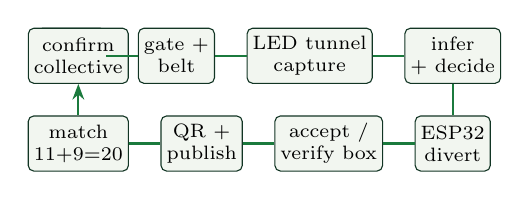
\begin{tikzpicture}[node distance=4mm, every node/.style={font=\scriptsize},
box/.style={rectangle,rounded corners=2pt,draw=herdark,fill=lightbg,minimum height=7mm,align=center,inner sep=2pt},
arr/.style={-{Stealth[length=2mm]},thick,hergreen}]
\node[box] (a) {create\\batch};
\node[box,right=of a] (b) {gate +\\belt};
\node[box,right=of b] (c) {LED tunnel\\capture};
\node[box,right=of c] (d) {infer\\+ decide};
\node[box,below=of d] (e) {ESP32\\divert};
\node[box,left=of e] (f) {accept /\\verify box};
\node[box,left=of f] (g) {QR +\\publish};
\node[box,left=of g] (h) {match\\11+9=20};
\node[box,above=of h] (i) {confirm\\collective};
\draw[arr] (a)--(b)--(c)--(d)--(e)--(f)--(g)--(h)--(i);
\end{tikzpicture}\caption{Fixed 10-step pipeline (condensed). Two outputs only; uncertain to verification.}\label{fig:pipeline}
\end{figure}
\subsection{Hardware bench}
Frame and \SI{60}{\centi\meter}--\SI{100}{\centi\meter} belt with \SI{12}{\volt} DC gear motor (\num{10}--\num{30}~RPM, PWM), matte-contrast cover, adjustable hopper gate, \SI{30}{\centi\meter} tunnel with \SI{5500}{\kelvin} LED strip, fixed UVC camera, servo flap chute, IR break-beam sense, red/green LEDs, mushroom NC e-stop in series with motor PSU coil + MCU sense line, guards, two food-contact boxes, \SI{120}{\milli\meter} \SI{12}{\volt} dust hood with G4/F7 filter, \SI{1}{\gram} scale. BOM \SI{675}{DT}--\SI{1350}{DT} excl.\ laptop ($\sim$\SI{1500}{DT} with laptop); each line needs three signed quotes before fact. Restart needs deliberate local button + UI resume; safe-boot leaves motor OFF.
Firmware speaks JSONL: divert/mode/stop/resume/hb. On divert it waits for the IR edge with \SI{3}{\second} jam timeout, pauses \SI{180}{\milli\second}, drives the flap (\ang{20} accepted / \ang{110} verify / \ang{65} home), emits sensed/diverted/fault. Heartbeat at \SI{1}{\hertz}.
\subsection{Vision: capture to decide}
Capture uses OpenCV at fixed exposure/WB. Preprocessing crops the ROI, denoises, builds an HSV green mask (\num{25},\num{30},\num{30}--\num{90},\num{255},\num{255}), keeps the largest contour, enforces the gate: exactly one contour, area \SI{1200}{px}--\SI{90000}{px}; else auto-verification, no guess. Inference runs MobileNetV3-Small \num{224}$\times$\num{224} ONNX on CPU over a colour-texture baseline; missing model falls back to a documented greenness heuristic so the bench never blocks. Decision:
\begin{equation}
\text{target}=\begin{cases} \text{accepted} & \text{pred=accepted} \wedge \text{conf}\ge\tau \wedge \text{gate ok}\\ \text{verify} & \text{otherwise} \end{cases}
\end{equation}
with $\tau=\num{0.75}$ (\texttt{v0.1-0.75}) tuned on validation. Mode~A maps uncertainty to \texttt{stop\_alert} + red lamp; Mode~B to \texttt{divert\_verify}. Every portion logs image ref, prediction, confidence, target, threshold version; event UUID makes re-POSTs idempotent. Dataset: $\ge$\num{300} bench images/class, split by batch \num{70}/\num{15}/\num{15}, unseen test batch. Surrogate = pipeline smoke only, labelled ANALOGY.
\subsection{Marketplace: match, order, price, QR}
Matching is pure and testable (Alg.~\ref{alg:match}). Hard filters reject herb mismatch, unavailable status/quantity, grade below required, harvest-window violations, and missing QR, each with a stored reason. Survivors are scored ($0.35$~visual + $0.25$~date + $0.20$~delivery + $0.20$~price) and greedily combined to the requested grams. Mixed grades set a banner but keep separate lines --- never one uniform grade.
\begin{algorithm}[htbp]\caption{Hard-filter to rank to combine.}\label{alg:match}
\KwIn{request $R$, lots $L$}\KwOut{lines, total, partial flag, exclusions}
$cands\gets[\,]$, $excl\gets[\,]$
\ForEach{$\ell\in L$}{\If{$hard\_filter(R,\ell)$ ok}{$cands.push((score(R,\ell),\ell))$} \Else{$excl.push((\ell.id,reason))$}}
sort $cands$ descending\; $total\gets0$
\ForEach{$(s,\ell)\in cands$}{\If{$total\ge R.qty$} break\; $take\gets\min(\ell.avail,R.qty-total)$\; emit line $(\ell,take,s)$\; $total+=take$}
\end{algorithm}
Orders move \texttt{proposed} to per-producer accept to buyer confirm to \texttt{confirmed}, decrementing availability once and locking batches from double-sell; declines release reservations. Pricing: $C_{total}=\sum C_{prod,proc,pack,trans,fees}$, $M_{kg}=P_{sale}-C_{total}$, $M_{total}=Q\cdot M_{kg}$, red warning when $P_{sale}<C_{total}$, logged with disclaimer. Public page \texttt{/b/\textless id\textgreater} shows herb, batch, as-entered date, locality level, quantities, grade summary, timeline, two images under \SI{150}{\kilo\byte} --- no contacts, no price.
\section{Results and Discussion}
\subsection{Vision evaluation}
Table~\ref{tab:eval} is filled from \texttt{docs/evidence/eval\_results.json} (accuracy, per-class P/R, confusion matrix, false-accept rate, review rate, ms/image). Surrogate runs stay separate, labelled ANALOGY, never cited as performance. Raising $\tau$ lowers false accepts but raises review load; the frozen operating point \texttt{v0.1-0.75} is the validation knee, printed on every batch page.
\begin{table}[htbp]\caption{Bench held-out evaluation (fill from evidence JSON).}\label{tab:eval}\centering
\begin{tabular}{@{}lc@{}}\toprule
Metric & Value\\
\midrule
$n$ (test, unseen batch) & ---\\
Accuracy & ---\\
Precision (accepted / verify) & --- / ---\\
Recall (accepted / verify) & --- / ---\\
False-accept rate & ---\\
Review rate & ---\\
Latency (ms/image, CPU) & ---\\
Threshold & 0.75 (v0.1-0.75)\\
\bottomrule
\end{tabular}\end{table}
\subsection{Sorting, throughput, dust, QR}
Sorting counts come from portion events (accepted vs.\ verification grams, \SI{20}{\gram}/portion). Throughput is portions/minute over three \SI{5}{\minute} runs. Dust evidence is paired: ten pours before/after with white-wipe photos --- visible-dust reduction claimed; respiratory protection explicitly not claimed. QR robustness is \num{10}/\num{10} phone scans on the LAN URL. Listing~\ref{lst:portion} shows the idempotent portion call from the smoke test.
\begin{lstlisting}[language=Python,caption={Idempotent portion ingest (smoke-tested).},label={lst:portion}]
POST /api/batches/{bid}/portions?mode=B
{"id": "evt-fixed-001", "pred": "accepted",
 "conf": 0.9, "image_ref": "img.jpg"}
# retry same id -> {"idempotent": true, ...}
\end{lstlisting}
\subsection{Matching, pricing, usability}
All seven matching tests pass (T-M1 exact \num{11}+\num{9}=\num{20}~kg cover; T-M2 herb; T-M3 grade; T-M4 stale date; T-M5 zero availability; T-M6 missing QR; T-M7 mixed grades flagged, lines separate). API smoke end-to-end passes: seed to portions to Mode-A stop to finish QR to \SI{20}{\kilo\gram} request to \SI{20}{\kilo\gram} proposal to two producer accepts + buyer confirm to pricing \num{10.00}/\num{2.00}/\num{40}~DT to public page \num{200}. Pricing validation confirms arithmetic + below-cost warning. Usability with two producers + one buyer records task success, time, frictions (large buttons, French labels).
\subsection{Failures and limits}
Overlap and blur drive verification --- the gate correctly refuses to guess. Jams trigger the \SI{3}{\second} fault + red lamp. Field batches will re-tune $\tau$. Honesty limits: no moisture, chemical, microbial, or aroma sensing; harvest dates as-entered; prices are entered-cost estimates; dust data visual only.
\section{Conclusion and Future Work}
Phase~1 delivers a runnable offline slice: bench screening with two honest outputs, QR-identified batches, collective \num{11}+\num{9}=\num{20}~kg fulfilment with IDs preserved, transparent pricing --- measured, anonymous, six pages. What scales is the pattern (gate to infer to divert to identify to combine), not one threshold. Future work (Phase~2): hosted Postgres, OTP accounts, ratings, collection routing, mobile-money ledger, multi-herb models, Arabic RTL UI, field trial with moisture/hygiene checks off-platform. Bench, dataset card, evidence logs, and video freeze together for reproduction.
\begin{tcolorbox}[colback=white,colframe=hergold,title=Reproduce in 3 commands,fonttitle=\bfseries\small]
\texttt{cp .env.example .env \&\& docker compose up --build -d}\\
\texttt{pytest -q} \quad (matching 7/7 + API smoke green)\\
\texttt{python -m vision.eval --data data/raw/rosemary}
\end{tcolorbox}
\section*{Acknowledgments}
We thank the women producers who described sorting work, dust, and collective-sale needs, and the challenge organisers for the Track~2 framing. Bench components were sourced locally; quotes filed as planning estimates.
\begin{thebibliography}{9}
\bibitem{challenge2026} Women and Rural Agriculture Innovation Challenge, Call guidelines, 2026, 2~pp.
\bibitem{howard2019} A.~Howard et~al., ``Searching for MobileNetV3,'' in \textit{Proc.\ ICCV}, 2019.
\bibitem{opencv} G.~Bradski, ``The OpenCV library,'' \textit{Dr.\ Dobb's J.}, 2000.
\bibitem{onnx} ONNX Runtime developers, ONNX Runtime docs, 2024. [Online].
\bibitem{fastapi} S.~Ramirez, FastAPI documentation, 2024. [Online].
\bibitem{segno} M.~Kid, Segno QR library docs, 2024. [Online].
\bibitem{sqlalchemy} M.~Bayer, SQLAlchemy documentation, 2024. [Online].
\bibitem{alpaydin2020} E.~Alpaydin, \textit{Introduction to Machine Learning}, 4th ed.\ MIT Press, 2020.
\end{thebibliography}
\end{document}
